\documentclass{article}
\usepackage{graphicx}
\usepackage[utf8]{inputenc}
\usepackage[english]{babel}
\usepackage{listings}
\usepackage{amssymb}
\usepackage{amsmath}
\usepackage{mathtools}
\usepackage{bbold}
\usepackage{color}
\usepackage{float}
\usepackage{url}
\usepackage{fancyvrb}
\setlength{\parindent}{2em}
\usepackage[colorlinks,linkcolor = black, urlcolor=black, citecolor =  blue]{hyperref}
%\usepackage{graphicx}
\begin{document}
\title{Ising model with Monte Carlo simulations}
\author{Hao Lin}
\maketitle


\begin{center}
\small
$\mathbf{Abstract}$
\end{center}
{\small
There exists a phase transition between an ordered phase and a disordered phase in ferromagnetic materials at a certain critical temperature. This project studies this phase transition with a simple 2-dimensional Ising model. Interactions of spins at different lattice sites are simulated through Monte Carlo simulations. The simulations involve systems of different lattice sites at different temperatures. Mean energy, heat capacity, mean absolute magnetic moment and magnetic susceptibility are studied as functions of temperature, where signals of phase transitions are observed and the critical temperature is obtained. The numerically found critical temperature is in good agreement with the analytic result.
}

\section{Introduction}
Properties of magnets have been known and utilized empirically by humans for hundred of years. The strong magnetic field of a magnet is created by a great number of electron spins aligned with one another. This subtle order, however, can be disturbed and broken by thermal motions of the electrons themselves. It was shown by Pierre Curie that the magnetism can be completely lost at a critical temperature, also known as the \emph{Curie temperature}. That is, ferromagnetic materials can experience a phase transition from an ordered phase to a disordered one as temperature approaches the critical temperature. 

Ernst Ising developed a simple statistical model, the \emph{Ising model}, to describe the interactions between different spin domains inside ferromagnetic materials.\cite{textbook} In the absence of an external magnetic field, the Ising model takes into account the two-body \emph{nearest-neighbour} interactions, favouring spin alignment and penalizing misalignment. Ising models beyond 1-dimension exhibit phase transitions.\cite{video} 

In this project, a simple 2-dimensional Ising model and its phase transition are studied. The equilibrium configurations are approached and evolved through Monte Carlo simulations. By looking at the mean energy, heat capacity, mean absolute magnetic moment and magnetic susceptibility at different temperatures, we can observe phase transitions clearly and determine the critical temperature. We also investigate systems of various lattice sizes to study the scaling property of the numerically found critical temperatures.

Section 2 contains brief descriptions of the Ising model and the Metropolis algorithm. Section 3 shows various results from the numerical simulations and discusses them in details. Section 4 summarizes the findings of this project and concludes with further remarks. 

\section{Theories and methods}
\subsection{Ising model}
In the Ising model, the microscopic structure of ferromagnetic materials is abstracted as a \emph{d}-dimensional lattice. Each lattice site has a definite spin, \{+1, -1\}, with $2d$ nearest neighbours. Interactions exist only in pairs of nearest neighbours. Alignment of near spins is energetically favourable, and misalignment is discouraged. In this project, we focus on 2-dimensional $L\times L$ systems. Without an external field, the entire model can be summarized in a simple two-body Hamiltonian,
\begin{equation}
\label{ }
E = -J\sum_{<kl>}^{N} s_k s_l,
\end{equation}
with $s_k \in \{+1, -1\}$, $J > 0$ being the interaction strength, $<kl>$ indicating nearest pairs and $N$ the total number of pairs. \cite{notes} To remove boundary effects, we also employ the periodic boundary conditions.

\subsection{Metropolis algorithm}
The Metropolis algorithm was first proposed by \emph{Metropolis et al.} in 1953.\cite{Mpaper} It enables us to use a sequence of random samples to approximate a target probability distribution. 

In the context of the Ising model, the target probability distribution is the distribution of the canonical ensemble of different lattice spin configurations. While the probability of each spin configuration is proportional to the corresponding Boltzmann factor, $e^{-E/T}$, the normalization constant,
\begin{equation*}
Z = \sum_{i} e^{-E_i/T},
\end{equation*}
is hard to compute, rendering a direct sampling extremely difficult. 

The Metropolis algorithm bypasses such a difficulty, as its sampling rule is contingent on the \emph{ratio}  $r$ of the probabilities only
\begin{equation}
r = \frac{Pr(\texttt{proposed state})}{Pr(\texttt{current state})}.
\end{equation}
It is not necessary to normalize the probability distribution in advance. 

The sampling rule is that if $r \ge 1$, the new sampling proposal will be accepted; if $r < 1$, $r$ needs to be confronted with a random number $rand$ uniformly sampled from $[0, 1]$, and the proposal will be accepted only if $rand < r$.

The step-by-step Metropolis algorithm adapted to this project goes as follows.
\begin{Verbatim}[frame=single]
1. Initialize all the spins in the lattice either randomly or 
uniformly as "spin-up";
2. Propose a spin flip at a randomly chosen site and compute the 
corresponding change of energy;
3. Apply the sampling rule;
4. Update the spin flip and other quantities such as energy and 
magnetic moment, if the flip proposal is accepted;
5. Repeat steps 2-4. Start collecting the sample sequence, once 
stability/equilibrium is established.
\end{Verbatim}

A few things are worthy of attention. First, one should note that the initial state dose not 
affect the simulation in the long run, and therefore one is free to choose any initialization in principle. The initialization does affect how long it takes to stabilize though. Also, the change of energy $\Delta E \in \{-8J, -4J, 0, 4J, 8J\}$. To speed up the algorithm, one should automatically accept the proposed flip as long as $\Delta E \ge 0$ and pre-compute the Boltzmann factors for $-8J$ and $-4J$. Similarly, it is also unnecessary to scan the entire lattice to update the energy and magnetic moment. 

The implementation in C++ can be found in the corresponding Github directory.

\section{Results and discussion}

\subsection{Special case: $2\times2$ lattice}
While analytic results for large scale lattices are extremely difficult to obtain, we do have a minimal $2\times2$ case that is not so daunting to play with analytically. This special case has a total of 16 configurations, all of which can be easily enumerated. A lot of symmetries can also be exploited. 

For the sake of this project, we calculate first the partition function $Z$ as a function of temperature $T$, from which the mean energy $E$, the heat capacity $C_v$, the mean absolute magnetization  $\langle|M|\rangle$ and the magnetic susceptibility $\chi$ follow. Analytic results are listed below.
\begin{align}
\label{}
Z(T)\, =&\,\, 4[3+Cosh(8J/T)], \\
E\, =&\,\, \frac{-8Sinh(8J/T)}{3+Cosh(8J/T)}, \\
C_v\, =&\,\, \frac{64[1+3Cosh(8J/T)]}{T^2 [3+Cosh(8J/T)]^2}, \\
 \langle|M|\rangle\, =&\,\, \frac{2[2+exp(8J/T)]}{3+Cosh(8J/T)}, \\
\chi\, =&\,\, \frac{8[1+exp(8J/T)]}{T[3+Cosh(8J/T)]}.
\end{align}

\begin{table}[ht]
\caption{Analytic and numerical results at $T=1$}
\centering
\begin{tabular}{c c c c}
\hline\hline
 & Analytic & Numerical & Percent Difference (\%) \\
 \hline
 $E$ & -7.9839 & -7.9839 & 0 \\
 $C_v$ & 0.12833 & 0.12829 & -0.03 \\
  $\langle|M|\rangle$ & 3.9946 & 3.9946 & 0 \\
 $\chi$ & 15.973 & 15.965 & -0.05 \\
 \hline
\end{tabular}
\end{table}

\emph{Table 1} compares results from both the analytic expressions and the numerical simulations, in the case of a $2\times2$ lattice at $T=1$. The numerical results agree very well with the analytic ones. It is found that it takes at least $O(10^5)$ Monte Carlo cycles to achieve a reasonable agreement. Also, the convergence of $C_v$ and $\chi$ is significantly slower than that of $E$ and  $\langle|M|\rangle$. It is due to the fact that $C_v$ and $\chi$ pertain to the variances of $E$ and  $\langle|M|\rangle$, containing \emph{finer} details of the equilibrium distribution. The numerical values display in \emph{Table 1} are obtained with $O(10^7)$ cycles.

\subsection{The road toward equilibrium}
While the Metropolis algorithm drives the system toward equilibrium, it is understood that the establishment of equilibrium is not instantaneous and does take a sizable amount of time. In this section, we investigate whether and how initialization and temperature may affect the number of Monte Carlo cycles to reach equilibrium for a $20\times20$ lattice. 

The simulations are run under 4 different conditions: 1) T=1 with uniform initialization; 2) T=1 with random initialization; 3) T=2.4 with uniform initialization; 4) T=2.4 with random initialization. Under each condition, a total of 5 quantities are scrutinized, namely $E$, $C_v$, $\langle|M|\rangle$, $\chi$ and the acceptance rate. Plots against number of Monte Carlo cycles are displayed as follows.

\begin{figure}[h]
\begin{center}
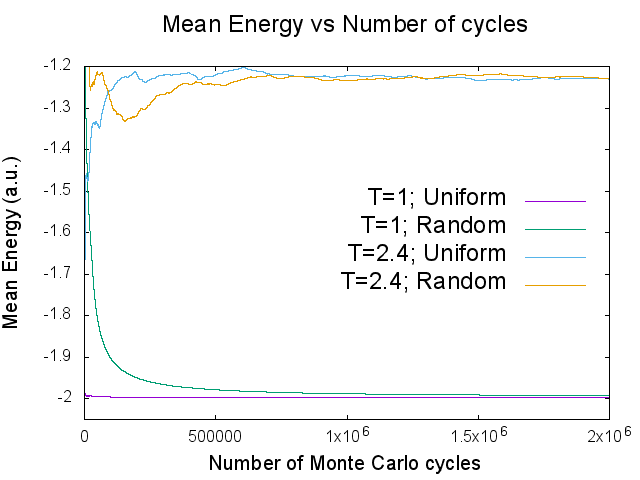
\includegraphics[width=0.8\textwidth]{E.png}
\caption{$E$ vs cycle number}
\end{center}
\end{figure}

\begin{figure}[H]
\begin{center}
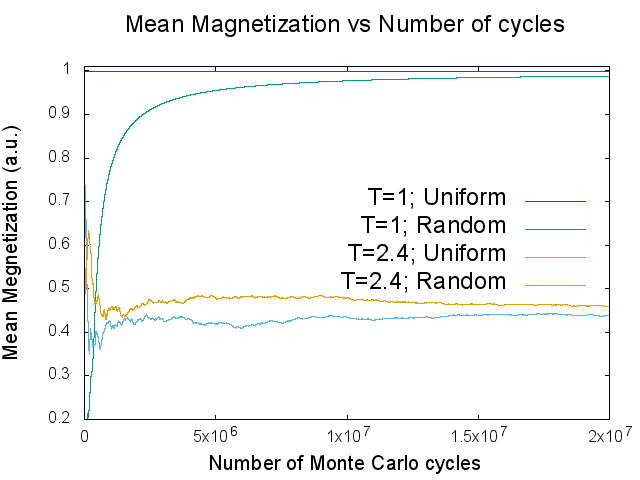
\includegraphics[width=0.8\textwidth]{M.png}
\caption{$\langle|M|\rangle$ vs cycle number}
\end{center}
\end{figure} 

At $T=1$, the uniform initialization is extremely close to the most probable configurations, and thus the equilibration process is almost instantaneous. In contrast, with a random initialization, the system needs a lot more spin flips to reach the most probable configurations. At $T=2.4$, a random initialization has more resemblance to the most probable configurations. However, the equilibration processes of the two initializations have roughly the same pace, taking $O(10^4)$ cycles toward equilibrium.

It can be observed from Figure 1 that the stable mean energy values can be reached after sufficiently many Monte Carlo cycles regardless of the conditions. More importantly, the convergent values of mean energy are independent of initializations. Figure 2 tells a similar yet different story: the convergence of mean magnetization can be reached, but there might exist inconclusive evidence of dependence on initialization. Such a spurious dependence should be expected to disappear if more Monte Carlo cycles are used. Comparing Figure 1 and Figure 2, we assert that $\langle|M|\rangle$ is a more sensitive indicator of equilibrium than $E$, and that if an initialization resembling the most likely configurations is chosen, it takes roughly $O(10^4)$ cycles to reach a reasonable approximation of the equilibrium.  

\begin{figure}[H]
\begin{center}
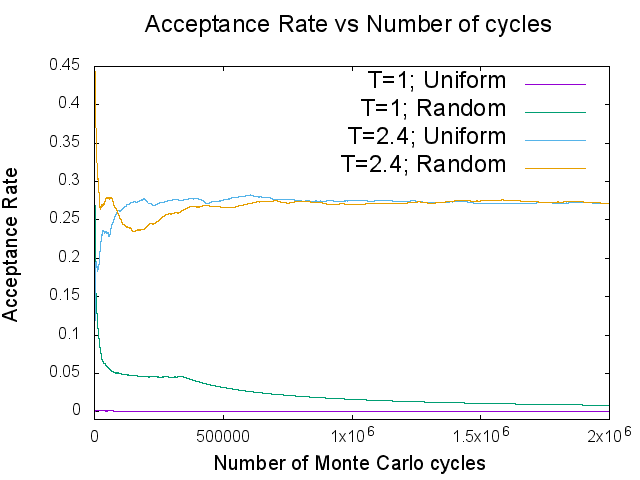
\includegraphics[width=0.8\textwidth]{Accept.png}
\caption{Acceptance rate vs cycle number}
\end{center}
\end{figure}

From Figure 3, we see that the stable acceptance rate is mostly a function of temperature. At equilibrium, the acceptance rate at $T=1$ is vanishingly small while that at $T=2.4$ is approximately 0.27. As the temperature increases, the acceptance rate also increases. This is expected and understood. In the sampling rule, the probability ratio goes like $e^{-\Delta E/T}$. Moves with $\Delta E \sim T$ have a non-negligible chance of acceptance even at equilibrium. The higher the temperature is, the more fluctuations the system has around equilibrium, and hence the higher the acceptance rate is.

\subsection{Energy probability distribution}
In this section, we look at the energy probability distributions $P(E)$ for a $20\times20$ lattice system at both $T=1$ and $T=2.4$. Data are accumulated after a sufficient number of Monte Carlo cycles, which ensures the approximate equilibrium has been reached. Below are plots of the energy probability distributions for the two temperatures. Note that the energy has been normalized to the \emph{energy per spin}.

\begin{figure}[h]
\begin{center}
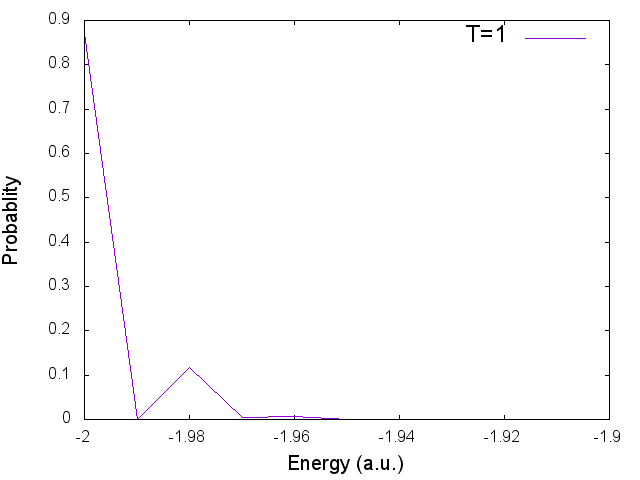
\includegraphics[width=0.8\textwidth]{T1.png}
\caption{Energy probability distribution at $T=1$ for a $20\times20$ lattice.}
\end{center}
\end{figure}

\begin{figure}[h]
\begin{center}
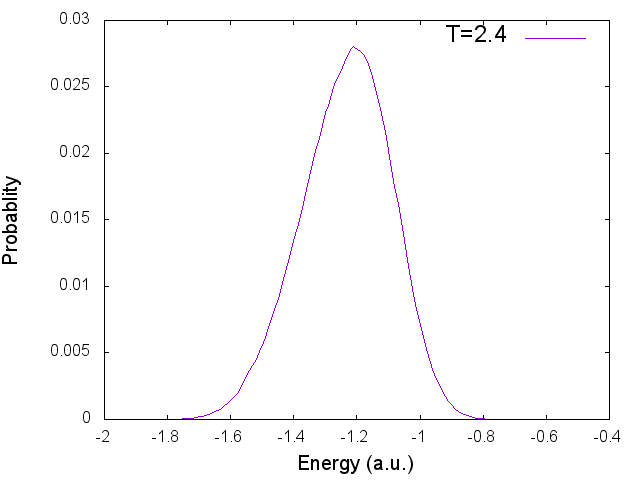
\includegraphics[width=0.8\textwidth]{T24.png}
\caption{Energy probability distribution at $T=2.4$ for a $20\times20$ lattice.}
\end{center}
\end{figure}

At very low temperature such as $T=1$, the probability density distribution is highly peaked at the lowest possible energy (ground state energy) with an exponentially decaying tail. It suggests that the system is essentially frozen in the ground state. The computed energy variance is also negligibly small, indicating very small fluctuations in the system. 

Above the critical temperature at $T=2.4$, the system can explore more energetic states. The peak of the distribution is shifted to higher energy, and the spread of the distribution is more evident and symmetric, resembling a Maxwell-Boltzmann distribution. The computed energy variance is significantly larger compared with the low temperature case. At high temperature, the system tend to exchange energy with the reservoir and jump between states with different energies much more actively.

The energy variance can be obtained from either direct calculations of the data
\begin{equation*}
\sigma_{E}^2 = \frac{1}{N}\sum_{cycles}E_{i}^{2} - \big(\frac{1}{N}\sum_{cycles}E_{i}\big)^2,
\end{equation*}
or the probability distribution
\begin{equation*}
\sigma_{E}^2 = \sum_{bins}E_{i}^{2}P(E_i) - \big(\sum_{bins}E_{i}P(E_i)\big)^2.
\end{equation*}

\begin{table}[ht]
\caption{Comparison of energy variance}
\centering
\begin{tabular}{c c c}
\hline\hline
 & Direct Cacl. & Prob. Dist. \\
 \hline
 $T=1$ & 5.802$\times10^{-5}$ & 5.802$\times10^{-5}$\\
 $T=2.4$ & 0.02024 & 0.02024 \\
 \hline
\end{tabular}
\end{table}

With a sufficiently fine binning ($\Delta E$ = 0.01), the energy variances computed from the probability distribution agree almost exactly with those found from direct calculations in both cases. It assures us that the probability distribution is correct, and that the sampling sequence generated by the Metropolis algorithm indeed provides us a very good approximation of the target distribution. 

\subsection{Phase transition}

The phase transition in this 2-dimensional Ising model is of the \emph{2nd order}. Therefore, at a certain critical temperature $T_c$, we expect to see \emph{inflection points} in $E$ and $\langle|M|\rangle$, and complete divergences in $C_v$ and $\chi$. In fact, it can be shown theoretically that the divergence behaviour of a second-order phase transition $\xi$ near $T_c$ is
\begin{equation}
\xi(T) \sim |T_c - T|^{-\nu},
\end{equation}
with $\nu > 0$ being some critical exponent. \cite{textbook} \cite{notes}

In order to investigate the phase transition from an ordered phase to a disordered phase of the lattice spins, we plot $E$, $C_v$, $\langle|M|\rangle$, $\chi$ as functions of temperature $T \in [2.2, 2.35]$ for varying square lattice size $L \in \{20, 40, 60, 80, 100\}$. 

\begin{figure}[h]
\begin{center}
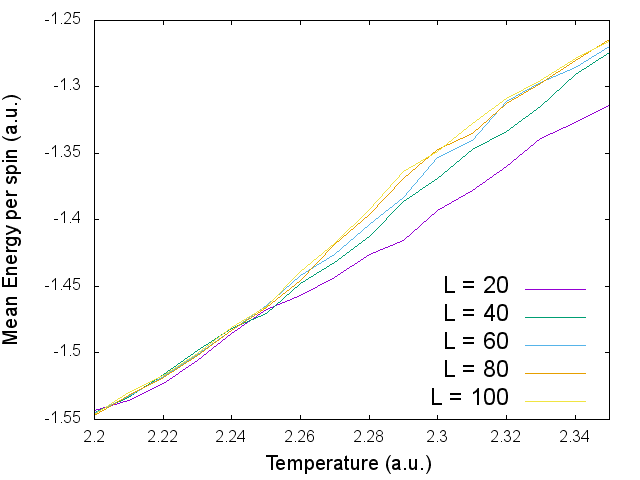
\includegraphics[width=0.8\textwidth]{PTE.png}
\caption{Energy per spin as a function of temperature. The divergence of the bundle of curves around $T=2.25$ indicates the set-in of the phase transition. The larger the lattice size, the more rapidly the energy grows around $T=2.27$, which is another indication of the phase transition.}
\end{center}
\end{figure}

\begin{figure}[h]
\begin{center}
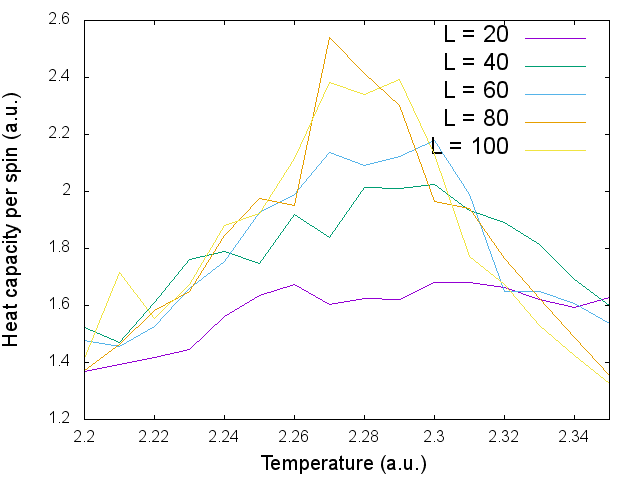
\includegraphics[width=0.8\textwidth]{PTCv.png}
\caption{Heat capacity per spin as a function of temperature. The peaks are increasingly higher as the lattice size increases, clearly suggesting a phase transition around $T=2.27$.}
\end{center}
\end{figure}

\begin{figure}[H]
\begin{center}
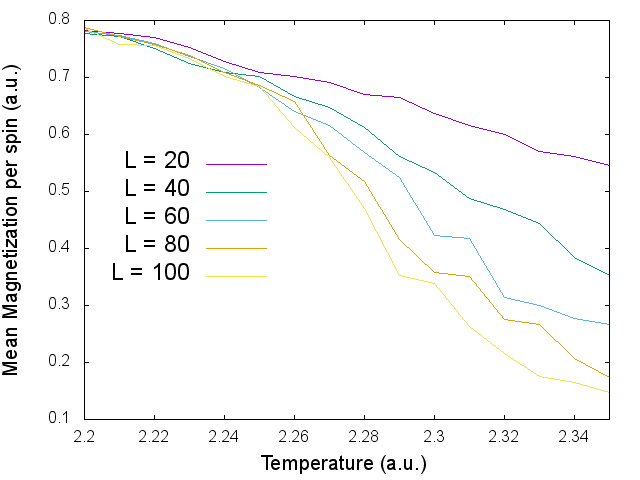
\includegraphics[width=0.8\textwidth]{PTM.png}
\caption{Mean Magnetization per spin as a function of temperature. Similar to the energy plot, the bundle starts to diverge at $T=2.25$. The greater the lattice size, the quicker the fall-off is. With $L=100$, we observe the greatest fall-off (inflection) around $T=2.27$. }
\end{center}
\end{figure}

\begin{figure}[H]
\begin{center}
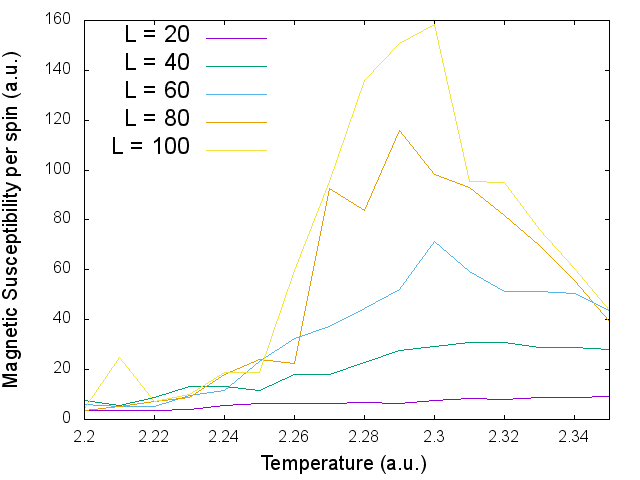
\includegraphics[width=0.8\textwidth]{PTChi.png}
\caption{Magnetic susceptibility per spin as a function of temperature. Note that the redifined $\chi = \frac{1}{T} \big( \langle M^2\rangle - \langle|M|\rangle^2\big)$ is used. The increasingly higher peaks again indicate a phase transition around $T=2.29$. The overestimation of $T_c$ might be due to the redefinition of $\chi$.}
\end{center}
\end{figure}

All four plots provide evidence for a phase transition with a critical temperature $T \in [2.25, 2.29]$. With the use of a larger lattice size, the inflectional behaviour for $E$ and $\langle|M|\rangle$ is more prominent, and the divergence peaks for $C_v$ and $\chi$ reach higher. It is easier to read off the critical temperature from plots and data of $C_v$ and $\chi$ for $L=100$, which yield the results in Table 3.

\begin{table}[ht]
\caption{Critical temperatures for $L=100$}
\centering
\begin{tabular}{c c c}
\hline\hline
 & from $C_v$ & from $\chi$ \\
 \hline
 $T_c$ & 2.28 & 2.30\\
 \hline
\end{tabular}
\end{table}

The values found are rather comparable to the analytic value by $T_c = 2.269$ by Lars Onsager.\cite{notes} It should be pointed out the staggering behaviours of the curves of $C_v$ and $\chi$ do pose difficulty in identifying the critical temperature. We expect it to be due to numerical fluctuations and can be removed should we use more Monte Carlo cycles. 

More notably, the critical temperature identified from the \emph{redefined} $\chi$ shifts toward the high end. Such a behaviour was not observed, when the normal definition of $\chi$ were used. The comparison between two different defintions of $\chi$ in the case of a $100\times100$ lattice is shown in Figure 10. With the normal definition of $\chi$, the reproduced critical temperature is around $T_c =2.26$, more comparable to the analytic value. The new definition does generate a smoother curve though.

\begin{figure}[H]
\begin{center}
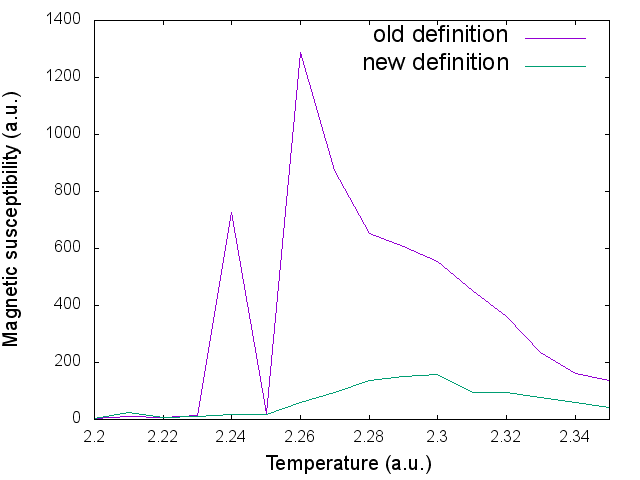
\includegraphics[width=0.8\textwidth]{compare.png}
\caption{Magnetic susceptibility per spin as a function of temperature. Two different definitions of $\chi$ are compared.}
\end{center}
\end{figure}

\subsection{Extraction of $T_c$ in the thermodynamic limit}
As we have seen from the previous results and discussions, $T_c$ indeed behaves as a function of the lattice size $L$. The true critical temperature $T_C$ should be understood in the thermodynamic limit as \cite{notes}
\begin{equation}
T_C = \lim_{L \to \infty} T_c(L). 
\end{equation}

It can be shown that there exists such a scaling law
\begin{equation}
T_c(L) = T_C + aL^{-1/\nu}
\end{equation}
with $\nu = 1$.\cite{notes}

We summarize values of $T_c(L)$ found from of $C_v(T)$ in the simulations in the following table. The values are found by averaging the temperatures of the two greatest $C_v$.

\begin{table}[ht]
\caption{Critical temperatures for different $L$}
\centering
\begin{tabular}{c c c c c c}
\hline\hline
 L & 40 & 60 & 80 & 100 & 140\\
 \hline
 $T_c$ & 2.29 &2.285 & 2.275 & 2.28 & 2.275 \\
 \hline
\end{tabular}
\end{table}

Noticing from Equation (9) that $T_c$ is \emph{linear} in $L^{-1}$ and that $T_C$ can be identified as the y-intercept, we perform a linear fit for $T_c(L^{-1})$ in \textbf{gnuplot} and find the fitted
\begin{equation}
T_C = 2.2689 \pm 0.003599.
\end{equation}
The corresponding plot is as follows.

\begin{figure}[H]
\begin{center}
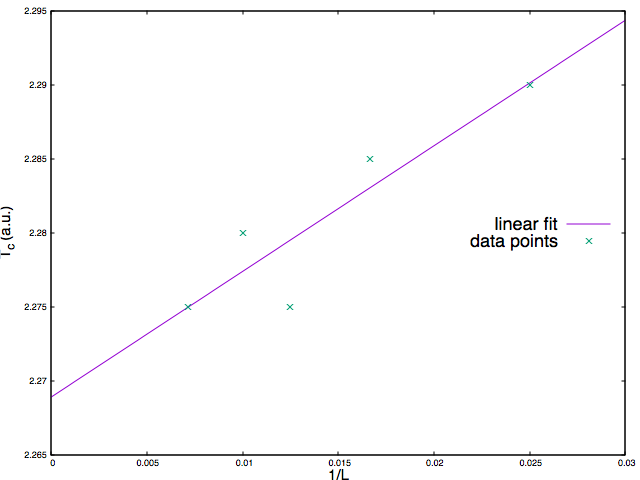
\includegraphics[width=0.8\textwidth]{F.png}
\caption{$T_c$ as a linear function of $1/L$}
\end{center}
\end{figure}

The fitted $T_C = 2.2689 \pm 0.003599$ is in good agreement with the expected value $2.269$.

\section{Summary and remarks}
This project explores the phase transition of ferromagnetic materials from an ordered magnetic phase to a disordered phase through a 2-dimensional Ising model. The Metropolis algorithm is employed to perform Monte Carlo simulations on lattices of spins. The systems evolve toward equilibria at different temperatures, and the Metropolis algorithm provides us with a useful sample of configurations at equilibrium. We have been able to calculate many thermodynamical quantities from the sample. The calculations and plots show clear signs of phase transitions at a definite temperature, confirming the correctness and success of both the Ising model and the Metropolis algorithm. Through the scaling properties, we obtain a fitted critical temperature in the thermodynamic limit, which agrees very well with the exact result. 

The Ising model is an extraordinarily elegant and simple model with a one-line long Hamiltonian. In the absence of an external field, the Hamiltonian itself manifests spin symmetry. Such a symmetry, however, can be broken by even the slightest external field. The two-body interactions are in favour of aligned spins, which is consistent with the existence of domains in ferromagnetic materials. Thermal motions are introduced through Monte Carlo simulations at different temperatures. It is the combat between the preference for an ordered phase and the random thermal motions that conspires to the phase transition. One can hardly not be in awe of such a simplistic yet powerful model. 

Incidentally, the Ising model can be \emph{approximated} by a mean-field approach. At each lattice site, the interaction depends only on the sum of nearest-neighbour magnetic moments. If neighbouring magnetic moments are replaced by a global mean magnetization, we will have a mean field approximation of the Ising model. A self-consistent equation can be set up, from which the critical temperature can be solved for.\cite{video} Obviously, the higher the dimension is, the better the mean field approximation would be. To a certain degree, this explains why only Ising models with dimension $\ge 2$ exhibit phase transitions.

\begin{thebibliography}{1}

\bibitem{textbook} Morten Hjorth-Jensen. {\em Computational Physics.} Lecture Notes Fall 2015.

\bibitem{notes} Morten Hjorth-Jensen. {\em Project 4 Ising Model and Statistical Physics.} \url{https://compphysics.github.io/ComputationalPhysicsMSU/doc/Projects/2017/Project4/IsingModel/pdf/IsingModel.pdf}

\bibitem{video} Leonard Susskind. {\em Statistical Mechanics Lecture 10.} (lecture video) \url{https://www.youtube.com/watch?v=IWtcFAP3ju4&index=10&list=PLXLSbKIMm0kjxyp45FIY62XNgHk4ywSaH}

\bibitem{Mpaper} Metropolis, Nicholas, et al. {\em Equation of state calculations by fast computing machines.} \textit{The journal of chemical physics} 21(6) (1953): 1087-1092.

\end{thebibliography}



\section*{Supplementary Material}   %asterisk * removes numbering
All source codes, raw data and plots can be found in the GIT repository: 
\url{https://github.com/Gartenzwerg/CompPhys/tree/master/Project4}

\end{document}